\chapter{Réalisation}
\label{chap:realisation}

Ce chapitre présente la réalisation des deux solutions. Après une description de l'environnement de travail, nous présentons le déploiement et le paramétrage du \ac{LIMS} au \ac{CTAA}, les interfaces du module de traçabilité, les tests de validation et la formation des utilisateurs. Nous exposons ensuite l'étude des équipements de Pharmaghreb, la réalisation du module d'acquisition et ses tests.

%-------------------------------------------------------------
\section{Environnement de travail}
%-------------------------------------------------------------

Le choix des outils a été guidé par la compatibilité avec l'existant (le \ac{LIMS} de BQube ITs repose sur \ac{PHP} et PostgreSQL), la fiabilité et l'adéquation aux besoins de chaque solution. Le tableau~\ref{tab:environnement} résume les technologies et les outils utilisés.

% À VÉRIFIER : outils de développement embarqué réellement utilisés.
\begin{table}[H]
\centering
\renewcommand{\arraystretch}{1.25}
\begin{tabularx}{\textwidth}{|p{3.6cm}|Y|}
\hline
\enteteligne \entete{Technologie / outil} & \entete{Rôle dans le projet} \\ \hline
\multicolumn{2}{|l|}{\cellcolor{bleuclair}\textbf{Module de traçabilité (CTAA)}} \\ \hline
HTML et CSS & Structure et mise en forme de l'interface : zone de saisie, choix du mode de recherche, tableaux de résultats \\ \hline
JavaScript et AJAX & Récupération de la chaîne lue par la douchette, envoi asynchrone au serveur et affichage dynamique des résultats \\ \hline
PHP & Back-end : identification du type de code, construction des requêtes SQL et mise en forme des réponses JSON \\ \hline
JSON & Format d'échange des données entre le serveur et le navigateur \\ \hline
PostgreSQL 9.6 et SQL & Stockage des données du LIMS et requêtes de traçabilité \\ \hline
phpPgAdmin & Administration de la base, mise au point et vérification des requêtes \\ \hline
Douchette et imprimante d'étiquettes & Lecture des codes QR et codes-barres ; impression des étiquettes \\ \hline
\multicolumn{2}{|l|}{\cellcolor{bleuclair}\textbf{Module d'acquisition (Pharmaghreb)}} \\ \hline
NodeMCU ESP-12E & Carte de développement à base d'ESP8266 \\ \hline
IDE Arduino (cœur ESP8266) & Écriture, compilation et téléversement du programme embarqué \\ \hline
Bibliothèques Wi-Fi, I$^2$C, PN532 et LCD & Connexion réseau, point d'accès de configuration, serveur HTTP, pilotage des périphériques \\ \hline
Outil de schéma électronique & Conception du schéma de câblage (figure~\ref{fig:cablage}) \\ \hline
\end{tabularx}
\caption{Technologies et outils utilisés.}
\label{tab:environnement}
\end{table}

%-------------------------------------------------------------
\section{Déploiement et paramétrage du LIMS au CTAA}
%-------------------------------------------------------------

\subsection{Fonctionnalités mises en place}

Cette première version du \ac{LIMS} couvre les fonctionnalités suivantes :
\begin{itemize}
    \item \textbf{demandes d'analyses} : création et suivi des demandes, enregistrement des analyses demandées, fiches de réception ;
    \item \textbf{échantillons} : identification, enregistrement et suivi tout au long de leur cycle de vie ;
    \item \textbf{produits et analyses} : catalogue des produits, des catégories et des analyses associées ;
    \item \textbf{équipements et métrologie} : suivi des équipements, de leurs contrôles et de leurs étalonnages ;
    \item \textbf{habilitations} : suivi des compétences et des habilitations du personnel ;
    \item \textbf{traçabilité} : module développé dans le cadre de ce projet (section~\ref{sec:module-tracabilite}).
\end{itemize}

\subsection{Création des utilisateurs et des droits d'accès}

Nous avons créé les comptes utilisateurs et attribué à chacun un profil (administrateur, technicien, responsable qualité, service administratif) qui détermine ses droits d'accès. Chaque action enregistrée est ainsi rattachée à son auteur, ce qui renforce la sécurité et la traçabilité.

\subsection{Configuration des produits et des analyses}

Les produits ont été créés et classés par catégories et sous-catégories (préparations alimentaires, sirops, nectars de jus, etc.), puis les analyses correspondantes ont été regroupées en \emph{packs} et associées aux produits. La figure~\ref{fig:configuration} montre par exemple le pack « Identification des colorants synthétiques », qui regroupe dix-sept analyses. Le \ac{LIMS} relie ainsi automatiquement chaque échantillon aux analyses à réaliser.

\begin{figure}[H]
  \centering
  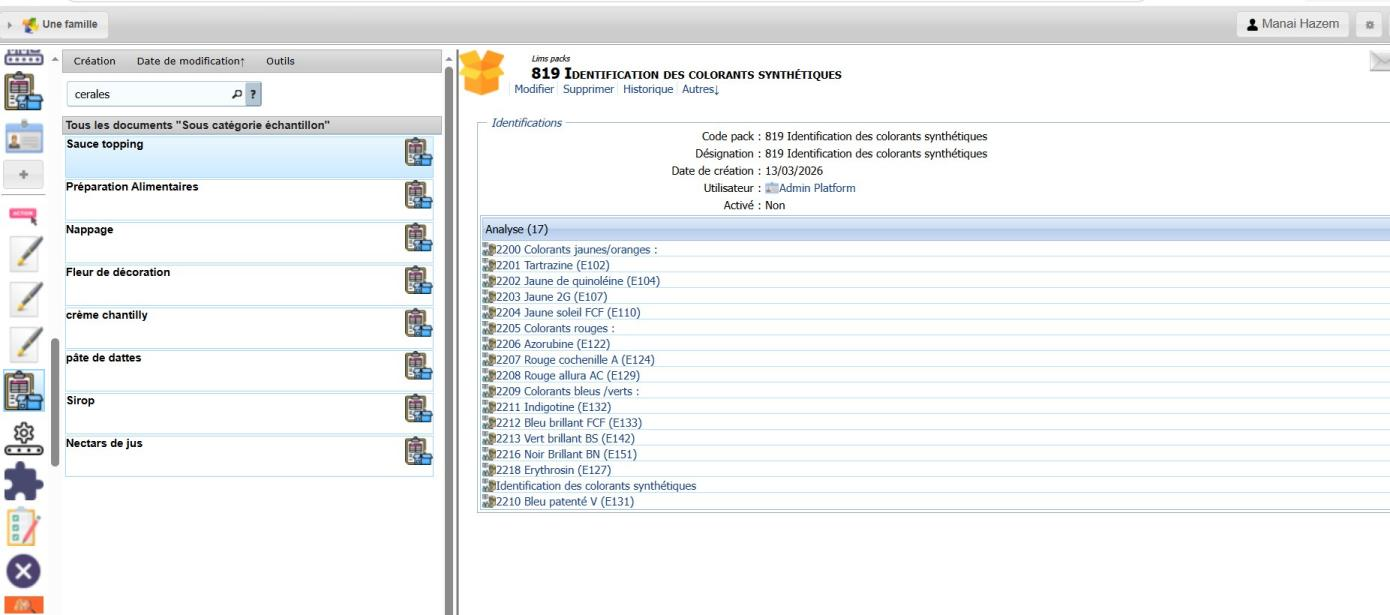
\includegraphics[width=\textwidth]{lims-configuration.png}
  \caption{Configuration des sous-catégories d'échantillons et d'un pack d'analyses.}
  \label{fig:configuration}
\end{figure}

\subsection{Gestion des demandes et étiquetage par code QR}

Le module de gestion des demandes (figure~\ref{fig:demandes}) permet d'enregistrer une demande client, d'y associer les échantillons et les analyses, de générer la fiche de réception et d'imprimer les étiquettes. Nous avons configuré l'imprimante et le format des étiquettes afin que chaque échantillon porte un identifiant unique et un code \ac{QR} (figure~\ref{fig:qr-echantillon}). Une fois apposée, l'étiquette relie directement l'échantillon physique à ses informations dans le \ac{LIMS}.

\begin{figure}[H]
  \centering
  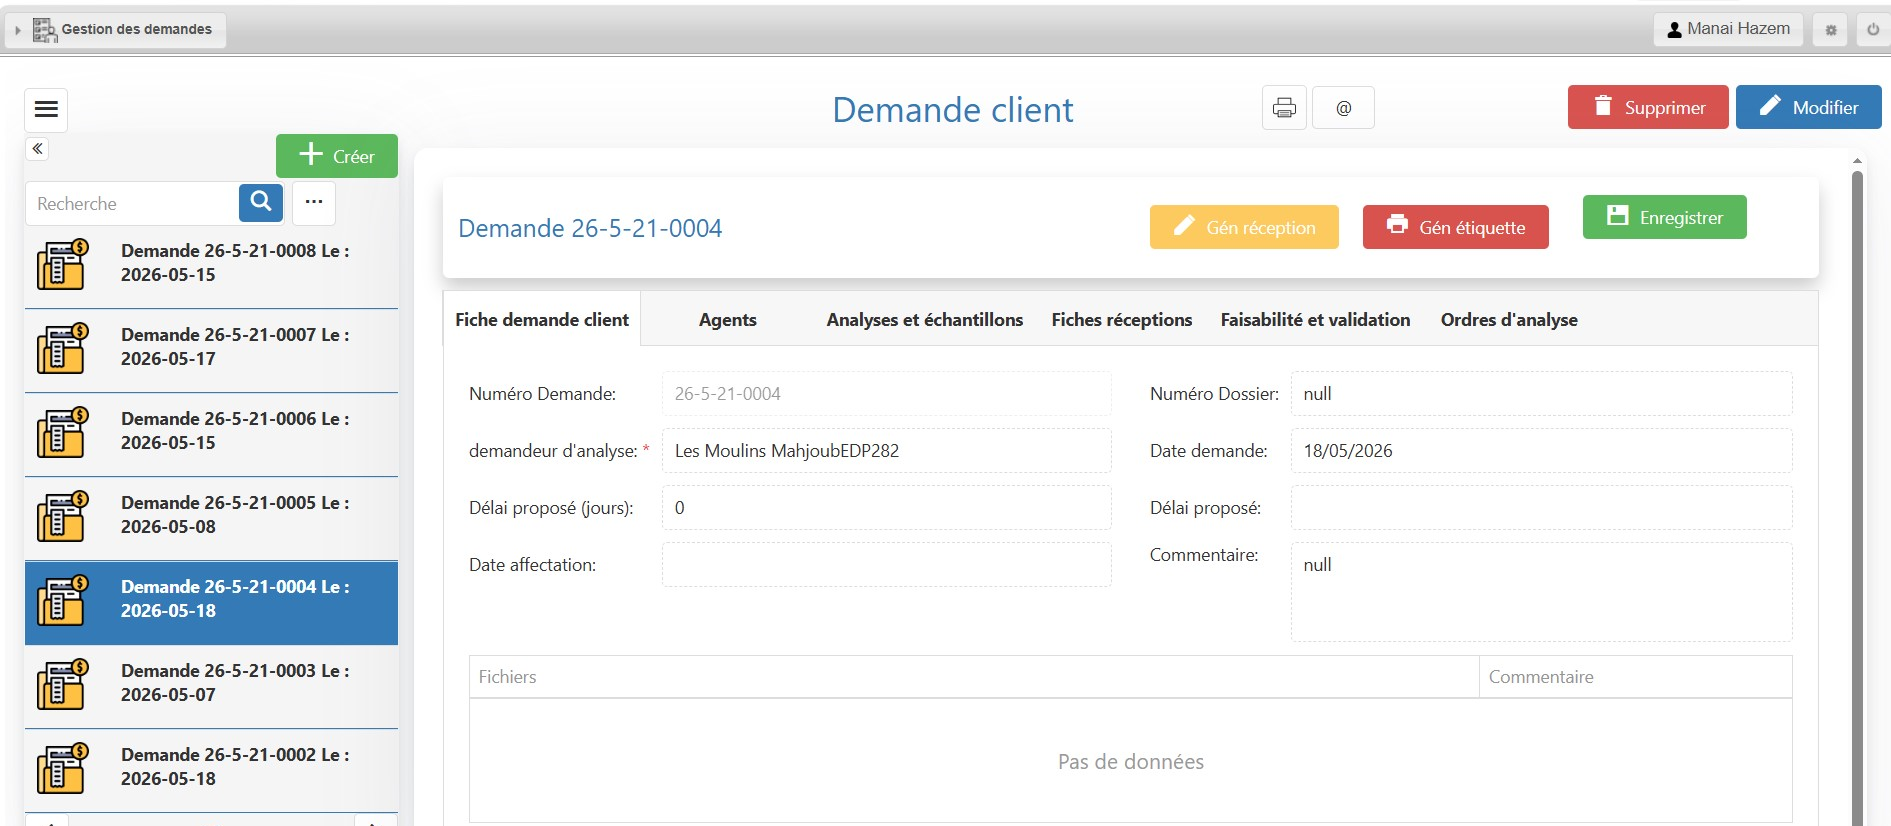
\includegraphics[width=\textwidth]{lims-demande-client.png}
  \caption{Module de gestion des demandes du LIMS.}
  \label{fig:demandes}
\end{figure}

\begin{figure}[H]
  \centering
  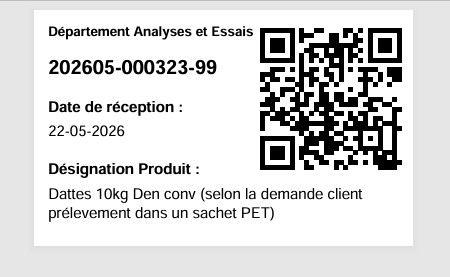
\includegraphics[width=0.5\textwidth]{etiquette-qr-echantillon.png}
  \caption{Étiquette d'échantillon avec code QR générée par le module de gestion des demandes.}
  \label{fig:qr-echantillon}
\end{figure}

Par rapport à l'ancienne étiquette (figure~\ref{fig:codebarre}), la nouvelle étiquette affiche la désignation complète du produit et se lit dans toutes les orientations. Le code \ac{QR} est pour l'instant limité au module de gestion des demandes ; les autres modules conservent le code-barres.

\subsection{Portail client}

Le portail client du \ac{CTAA} (figure~\ref{fig:portail}) complète le \ac{LIMS}. Il permet aux clients de déposer leurs demandes d'analyses, de consulter leurs devis et d'accéder à leurs rapports en ligne, ce qui répond au problème des déplacements identifié lors de l'analyse de l'existant.

\begin{figure}[H]
  \centering
  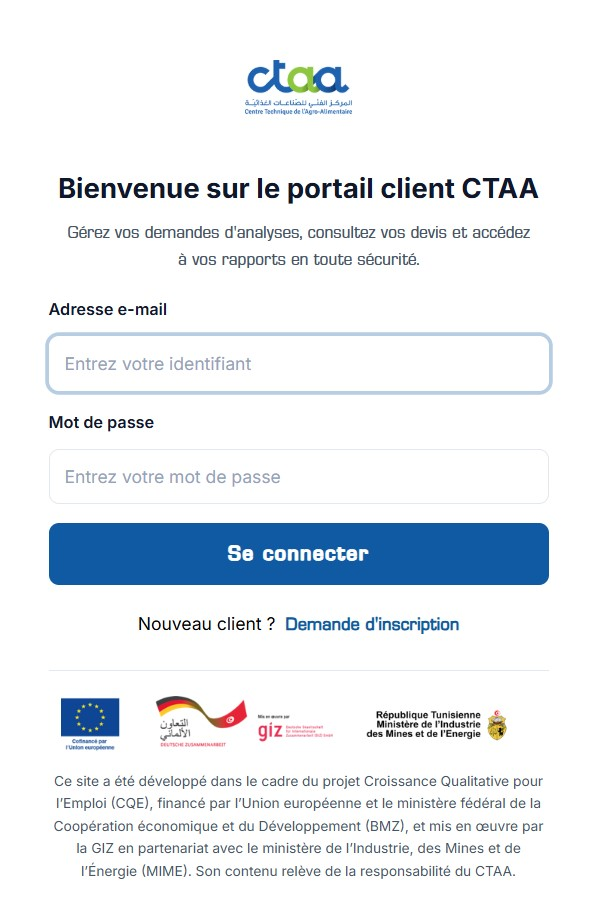
\includegraphics[width=0.45\textwidth]{portail-client-ctaa.jpg}
  \caption{Page de connexion du portail client du CTAA.}
  \label{fig:portail}
\end{figure}

%-------------------------------------------------------------
\section{Réalisation du module de traçabilité}
\label{sec:module-tracabilite}
%-------------------------------------------------------------

\subsection{Interface d'accueil}

L'interface du module (figure~\ref{fig:trace-accueil}) propose deux cases à cocher pour choisir le mode de recherche, « Code à barre » ou « Numéro de série », et un champ unique qui reçoit la lecture de la douchette ou une saisie manuelle.

\begin{figure}[H]
  \centering
  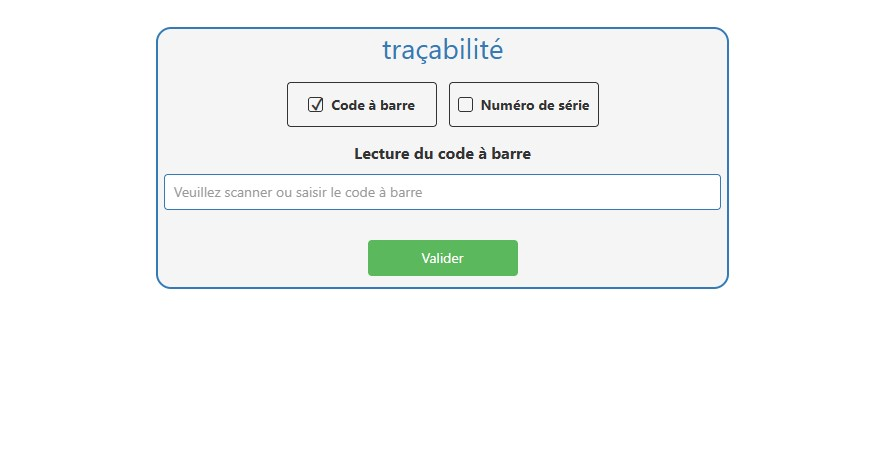
\includegraphics[width=0.75\textwidth]{trace-accueil.jpg}
  \caption{Interface d'accueil du module de traçabilité.}
  \label{fig:trace-accueil}
\end{figure}

\subsection{Traçabilité par code}

En mode « Code à barre », la lecture d'un code de préparation affiche le tableau de traçabilité correspondant : produit, emballage, numéro d'étiquette, lots utilisés, magasin, fournisseur et dates (figure~\ref{fig:trace-code}). Le code lu dans cet exemple est celui décomposé au tableau~\ref{tab:exemple-code}.

\begin{figure}[H]
  \centering
  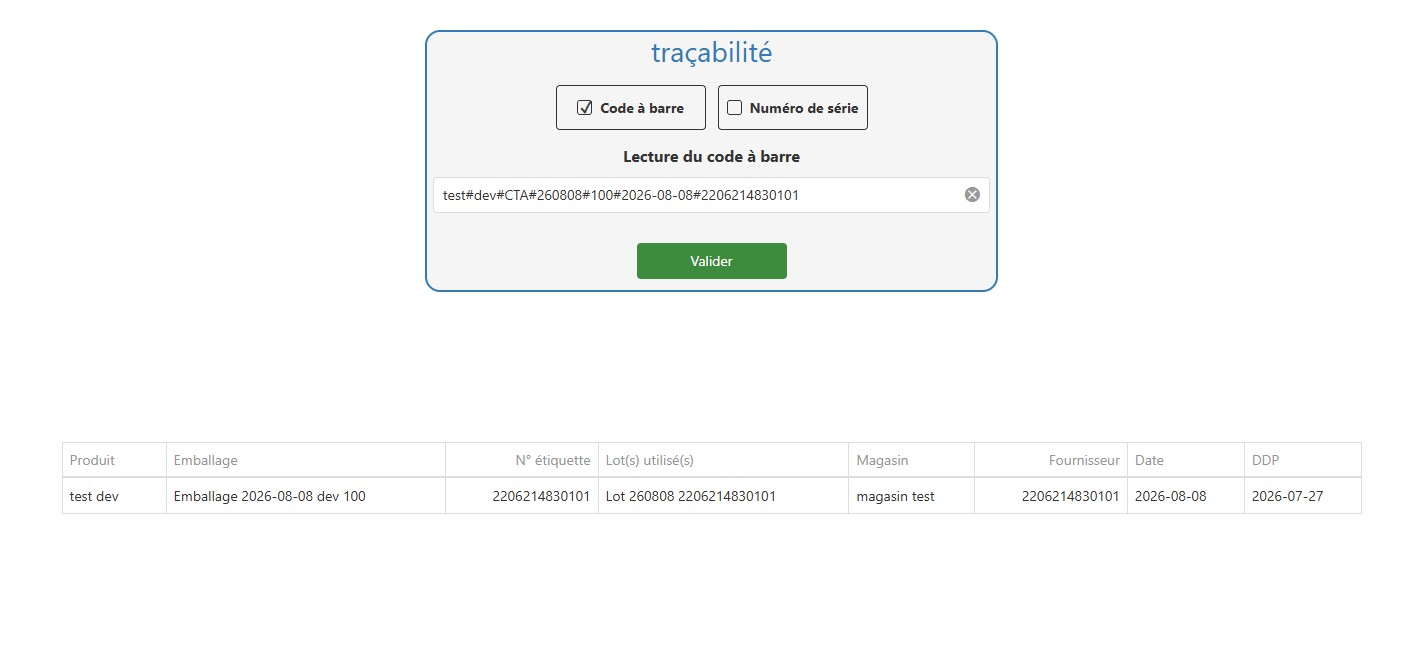
\includegraphics[width=\textwidth]{trace-code-barres.jpg}
  \caption{Traçabilité d'une préparation à partir de son code.}
  \label{fig:trace-code}
\end{figure}

\subsection{Traçabilité par numéro de série}

En mode « Numéro de série », la saisie du numéro de lot \texttt{CS07251350} affiche toutes les lignes de réception qui le concernent : numéro de réception, article, quantités demandée et reçue, \ac{DLC} et utilisateur ayant enregistré la réception (figure~\ref{fig:trace-serie}). Ce résultat est produit par la requête du listing~\ref{lst:requete-serie}, dont la figure~\ref{fig:requete-sql} montre la mise au point dans phpPgAdmin.

\begin{figure}[H]
  \centering
  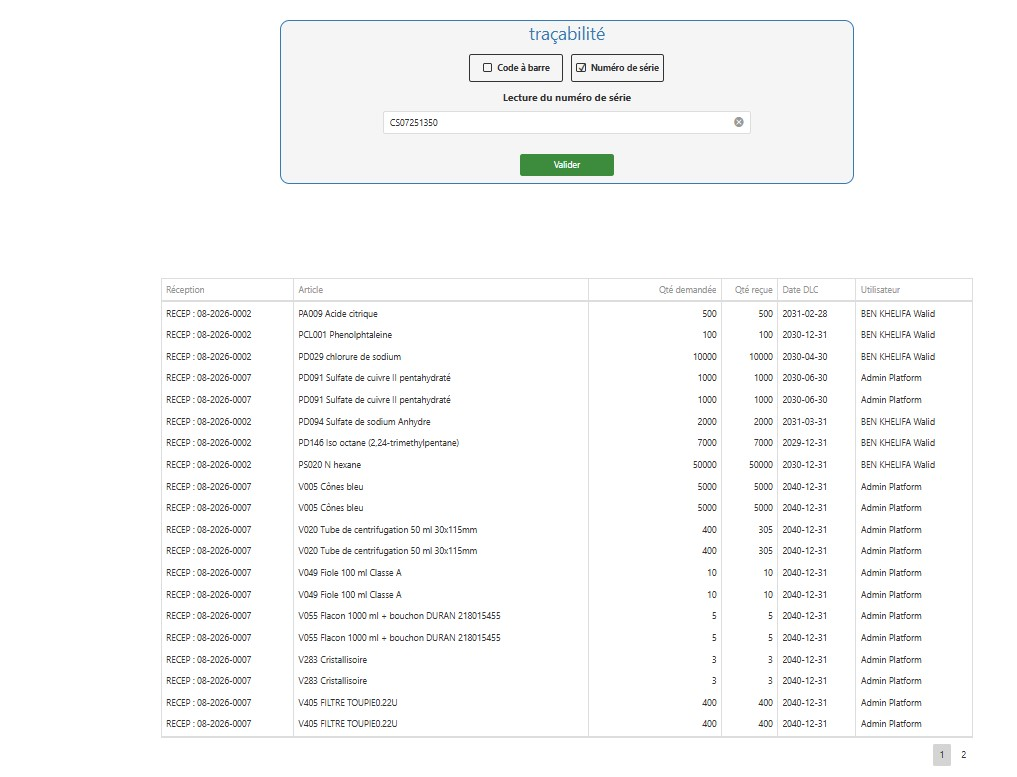
\includegraphics[width=\textwidth]{trace-num-serie.jpg}
  \caption{Traçabilité des réceptions à partir d'un numéro de série.}
  \label{fig:trace-serie}
\end{figure}

\begin{figure}[H]
  \centering
  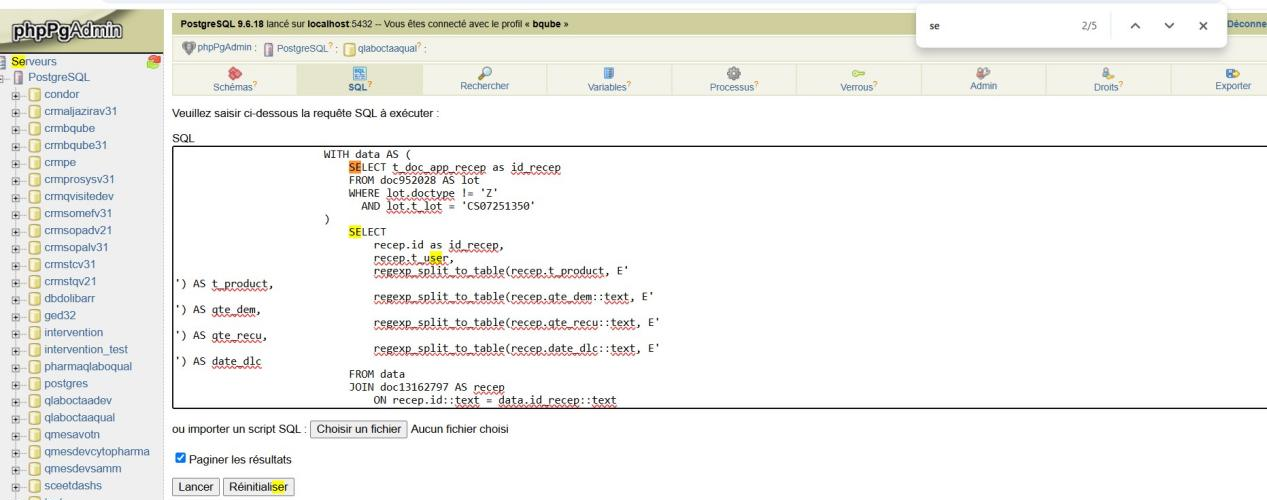
\includegraphics[width=\textwidth]{requete-sql-tracabilite.png}
  \caption{Mise au point de la requête de traçabilité dans phpPgAdmin.}
  \label{fig:requete-sql}
\end{figure}

\subsection{Gestion des erreurs}

Lorsque le code lu ne respecte aucune structure connue ou ne correspond à aucun élément de la base, le module affiche un message explicite invitant l'utilisateur à vérifier la valeur (figure~\ref{fig:trace-erreur}). L'utilisateur peut alors relancer la lecture sans quitter la page.

\begin{figure}[H]
  \centering
  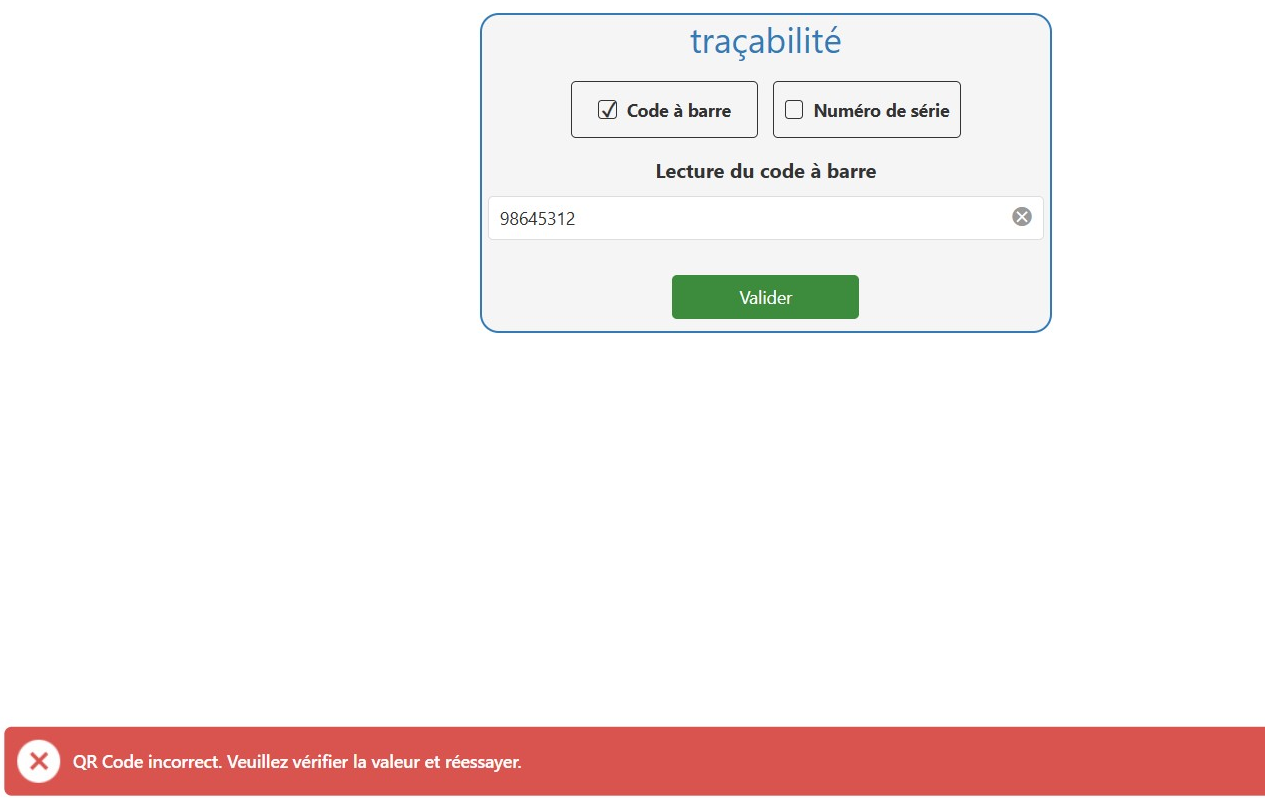
\includegraphics[width=0.85\textwidth]{trace-erreur.png}
  \caption{Message d'erreur affiché pour un code incorrect.}
  \label{fig:trace-erreur}
\end{figure}

\subsection{Extrait du code back-end}

La figure~\ref{fig:code-php} présente un extrait de la fonction \texttt{getDataTabLot} du back-end. On y retrouve les choix de conception décrits au chapitre~\ref{chap:conception} : résolution des familles de documents par leur nom (\texttt{getIdFromName}), lecture des paramètres dans \texttt{config.ini}, connexion à PostgreSQL, puis construction progressive de la clause de filtrage selon les critères reçus (numéro, composant, dates de début et de fin).

\begin{figure}[H]
  \centering
  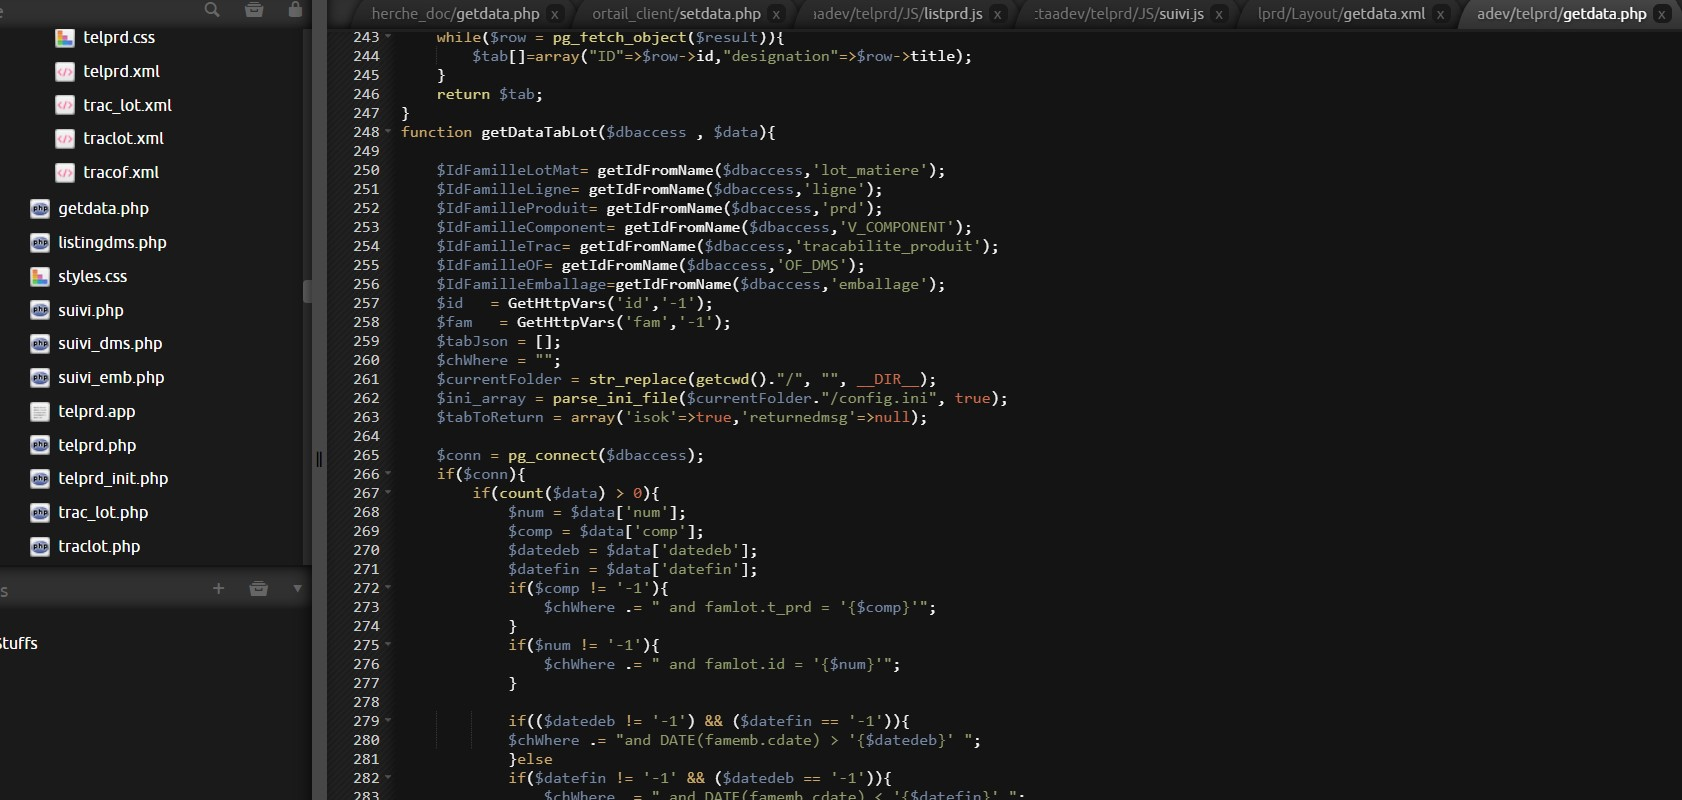
\includegraphics[width=\textwidth]{code-backend-php.png}
  \caption{Extrait du code PHP du back-end du module de traçabilité.}
  \label{fig:code-php}
\end{figure}

%-------------------------------------------------------------
\section{Tests et validation}
%-------------------------------------------------------------

Conformément au cycle en V, chaque fonctionnalité a été vérifiée par rapport aux besoins exprimés au chapitre~\ref{chap:analyse-besoins}. Le tableau~\ref{tab:tests-ctaa} présente les scénarios de test et leurs résultats. Les anomalies relevées lors d'une première série de tests ont été corrigées, puis l'ensemble des scénarios a été rejoué.

% À VÉRIFIER : compléter ou ajuster selon les tests réellement menés.
\begin{table}[H]
\centering
\renewcommand{\arraystretch}{1.25}
\begin{tabularx}{\textwidth}{|c|Y|Y|c|}
\hline
\enteteligne \entete{N°} & \entete{Scénario} & \entete{Résultat attendu} & \entete{Résultat} \\ \hline
T1 & Connexion avec chaque profil d'utilisateur & Accès limité aux fonctionnalités du rôle & Conforme \\ \hline
T2 & Création d'une demande et association des analyses d'un produit & Analyses du pack rattachées automatiquement & Conforme \\ \hline
T3 & Impression d'une étiquette puis lecture de son code QR & Identifiant lu correctement par la douchette & Conforme \\ \hline
T4 & Lecture d'un code de préparation valide (BF1) & Tableau de traçabilité de la préparation & Conforme \\ \hline
T5 & Saisie d'un numéro de série existant (BF2) & Liste des réceptions du lot & Conforme \\ \hline
T6 & Saisie d'un code mal formé (BF4) & Message « code incorrect » & Conforme \\ \hline
T7 & Code bien formé mais absent de la base (BF4) & Message d'erreur, aucune donnée affichée & Conforme \\ \hline
T8 & Comparaison des données affichées avec la base (phpPgAdmin) & Données identiques & Conforme \\ \hline
T9 & Consultation d'un historique incomplet & Affichage des seules opérations existantes, sans erreur & Conforme \\ \hline
\end{tabularx}
\caption{Scénarios de test du LIMS et du module de traçabilité.}
\label{tab:tests-ctaa}
\end{table}

%-------------------------------------------------------------
\section{Formation et accompagnement des utilisateurs}
%-------------------------------------------------------------

\subsection{Enjeux et objectifs}

La réussite d'un \ac{LIMS} ne dépend pas seulement de son paramétrage : elle repose aussi sur son appropriation par les utilisateurs. Un outil bien configuré mais mal maîtrisé reste sous-utilisé, et les anciennes habitudes (papier, fichiers Excel) risquent de revenir. Une part importante de la mission a donc été consacrée à la formation et à l'accompagnement du personnel du \ac{CTAA}, avec quatre objectifs :
\begin{itemize}
    \item rendre chaque utilisateur autonome sur les fonctionnalités liées à son rôle ;
    \item faire comprendre le passage d'un fonctionnement papier à un fonctionnement numérique et centralisé ;
    \item réduire les erreurs d'utilisation pendant les premières semaines ;
    \item recueillir les retours du terrain pour ajuster le système.
\end{itemize}

\subsection{Démarche suivie}

Les contenus ont été adaptés à chaque profil (tableau~\ref{tab:formation-profils}), et l'accompagnement s'est déroulé en quatre temps :
\begin{enumerate}
    \item \textbf{Préparation} : définition du contenu de chaque session et préparation d'exemples tirés des cas réels du laboratoire.
    \item \textbf{Formation fonctionnelle} : animation des sessions, avec un niveau de détail adapté au profil des participants.
    \item \textbf{Accompagnement sur le terrain} : assistance en temps réel des utilisateurs travaillant sur le \ac{LIMS}, notamment pour l'identification par code \ac{QR}.
    \item \textbf{Recueil des retours} : les remarques des utilisateurs ont révélé des écarts entre les processus prévus et les pratiques réelles, et ont servi à ajuster le paramétrage.
\end{enumerate}

\begin{table}[H]
\centering
\renewcommand{\arraystretch}{1.25}
\begin{tabularx}{\textwidth}{|p{3.1cm}|Y|Y|}
\hline
\enteteligne \entete{Profil} & \entete{Contenu et modalités} & \entete{Compétences acquises} \\ \hline
Administrateur & Session technique et accompagnement au paramétrage & Gestion des comptes, des rôles et des droits d'accès \\ \hline
Technicien de laboratoire & Sessions collectives et assistance sur le poste de travail & Enregistrement des échantillons, saisie des résultats, lecture des codes, consultation de la traçabilité \\ \hline
Responsable qualité & Session fonctionnelle et suivi en situation réelle & Suivi des analyses, de la traçabilité, des habilitations et des équipements \\ \hline
Service administratif & Session fonctionnelle courte & Consultation des rapports et suivi des demandes \\ \hline
\end{tabularx}
\caption{Formation des utilisateurs par profil.}
\label{tab:formation-profils}
\end{table}

\subsection{Difficultés rencontrées et solutions apportées}

Le passage au numérique a soulevé plusieurs difficultés :
\begin{itemize}
    \item \textbf{la résistance au changement} : certains utilisateurs étaient attachés aux supports papier ; nous avons mis en avant les bénéfices concrets pour leur travail (moins de ressaisies, recherche plus rapide) ;
    \item \textbf{des niveaux d'aisance informatique différents} : l'accompagnement individuel sur le poste de travail a complété les sessions collectives ;
    \item \textbf{des écarts entre le processus théorique et la pratique} : les retours du terrain ont conduit à des ajustements du paramétrage.
\end{itemize}

Au terme de cette phase, le \ac{LIMS} est intégré aux pratiques quotidiennes du laboratoire, et les utilisateurs perçoivent ses gains concrets : moins de ressaisies et un accès plus rapide à l'information.

%-------------------------------------------------------------
\section{Réalisation du module d'acquisition (Pharmaghreb)}
%-------------------------------------------------------------

\subsection{Étude de connectivité des équipements}

Avant de réaliser le module, nous avons étudié dix équipements du laboratoire de contrôle de Pharmaghreb : interfaces disponibles, protocoles supportés et tests de communication. Le tableau~\ref{tab:etude-equipements} présente les résultats. Il montre que les équipements récents peuvent être interrogés directement par Ethernet, alors que les autres ne disposent que d'une liaison \ac{RS-232}, d'où l'intérêt d'un module d'acquisition.

\begin{table}[H]
\centering
\small
\renewcommand{\arraystretch}{1.25}
\begin{tabularx}{\textwidth}{|p{3.9cm}|p{2.5cm}|Y|}
\hline
\enteteligne \entete{Équipement} & \entete{État} & \entete{Résultat et mode de communication} \\ \hline
Balance Mettler Toledo XPR205 & Communication testée & Ethernet et protocole MT-SICS \\ \hline
Balance Mettler Toledo XSR205 & Communication testée & Ethernet et protocole MT-SICS ; RS-232 et MT-SICS via le module d'acquisition développé \\ \hline
pH-mètre Mettler Toledo SevenExcellence & Communication testée & Ethernet, TCP/IP, via le service de communication Mettler (messages XML) \\ \hline
Titrateur volumétrique compact Karl Fischer V30 & Communication testée & Communication possible uniquement avec le logiciel Mettler LabX \\ \hline
Polarimètre Bellingham + Stanley ADP450 & Communication testée & Ethernet et protocole FTP pour le téléchargement des résultats \\ \hline
Spectromètre L1600300 (logiciel Spectrum) & Communication testée & Liaison Ethernet établie, sans réponse du logiciel Spectrum ; en attente du fournisseur \\ \hline
pH-mètre Mettler Toledo S230 & En attente d'un module ESP32 & RS-232 ou adaptateur USB/RS-232 (à tester) \\ \hline
pH-mètre Mettler Toledo SevenMulti S47 & En attente d'un module ESP32 & Second port RS-232, désactivé selon la documentation (à tester) \\ \hline
Appareil de point de fusion BUCHI M-565 & En attente d'un module ESP32 & RS-232 ou adaptateur USB/RS-232 (à tester) \\ \hline
\end{tabularx}
\caption{Résultats de l'étude de connectivité des équipements de Pharmaghreb.}
\label{tab:etude-equipements}
\end{table}

\subsection{Réalisation du prototype}

Le prototype a été assemblé selon le schéma de câblage de la figure~\ref{fig:cablage}, puis le programme embarqué a été développé selon l'organigramme de la figure~\ref{fig:organigramme}. La balance Mettler Toledo XSR205 a été retenue comme équipement de validation, car elle peut être interrogée à la fois par Ethernet et par \ac{RS-232} : cela permet de comparer les mesures obtenues par les deux voies.

\subsection{Tests du prototype}

Le tableau~\ref{tab:tests-prototype} présente les tests réalisés sur le prototype. Tous les scénarios sont conformes : le module est \textbf{complet et fonctionnel}, et il attend son déploiement sur site.

% À VÉRIFIER : ajuster selon les tests réellement menés.
\begin{table}[H]
\centering
\renewcommand{\arraystretch}{1.25}
\begin{tabularx}{\textwidth}{|c|Y|Y|c|}
\hline
\enteteligne \entete{N°} & \entete{Scénario} & \entete{Résultat attendu} & \entete{Résultat} \\ \hline
P1 & Envoi de la commande \texttt{S} à la balance XSR205 & Trame reçue et valeur décodée & Conforme \\ \hline
P2 & Pesée en cours de stabilisation & Valeur instable non enregistrée & Conforme \\ \hline
P3 & Présentation d'un badge NFC & Identifiant lu et associé aux mesures & Conforme \\ \hline
P4 & Premier démarrage sans réseau connu & Ouverture du point d'accès de configuration & Conforme \\ \hline
P5 & Connexion au réseau local & Adresse IP affichée sur l'écran LCD & Conforme \\ \hline
P6 & Appui de 5 s sur le bouton & Configuration Wi-Fi effacée & Conforme \\ \hline
P7 & Requête HTTP sur \texttt{/getData} & Dernière mesure renvoyée au format JSON & Conforme \\ \hline
\end{tabularx}
\caption{Scénarios de test du module d'acquisition.}
\label{tab:tests-prototype}
\end{table}

\subsection{État d'avancement}

Le module d'acquisition est réalisé et validé en laboratoire. Les prochaines étapes sont :
\begin{itemize}
    \item le déploiement du module sur le poste de pesée et sa validation en conditions réelles ;
    \item l'intégration des mesures au système d'information de Pharmaghreb, puis au \ac{LIMS} ;
    \item la connexion des équipements en attente, à l'aide de modules ESP32 ;
    \item le développement d'une interface de supervision centralisée.
\end{itemize}

%-------------------------------------------------------------
\section*{Conclusion}
\addcontentsline{toc}{section}{Conclusion}
%-------------------------------------------------------------

Ce chapitre a présenté la réalisation des deux solutions. Au \ac{CTAA}, le \ac{LIMS} a été paramétré et mis en service, l'étiquetage des échantillons par code \ac{QR} a été mis en place dans le module de gestion des demandes, et le module de traçabilité a été développé, testé et adopté grâce à la formation des utilisateurs. Chez Pharmaghreb, l'étude de connectivité de dix équipements a guidé la réalisation d'un module d'acquisition complet et testé, qui attend son déploiement.
